%!TEX root = main.tex
\section{Related Work\label{sec:related}}
% \todo[inline]{NOTE: Add related works on CV methods for object segmentation, what their problem is and why we need crowdsourcing responses (CITE GraphCut, CRFs)}
% \par As described in the introduction, accurate segmentations are essential for reliable object detection and tracking~\cite{sivic2005discovering,felzenszwalb2008discriminatively,viola2004robust,torralba2004sharing,torralba2003contextual,fe2003bayesian,Bearman2016}, necessitating the use of crowdsourcing to gather training data~\cite{AdrianaKovashka2016}. \agp{the previous sentence can be dropped if you have already talked about use cases for segmentation in the intro -- no need to repeat.}
\begin{figure}[h!]
\centering
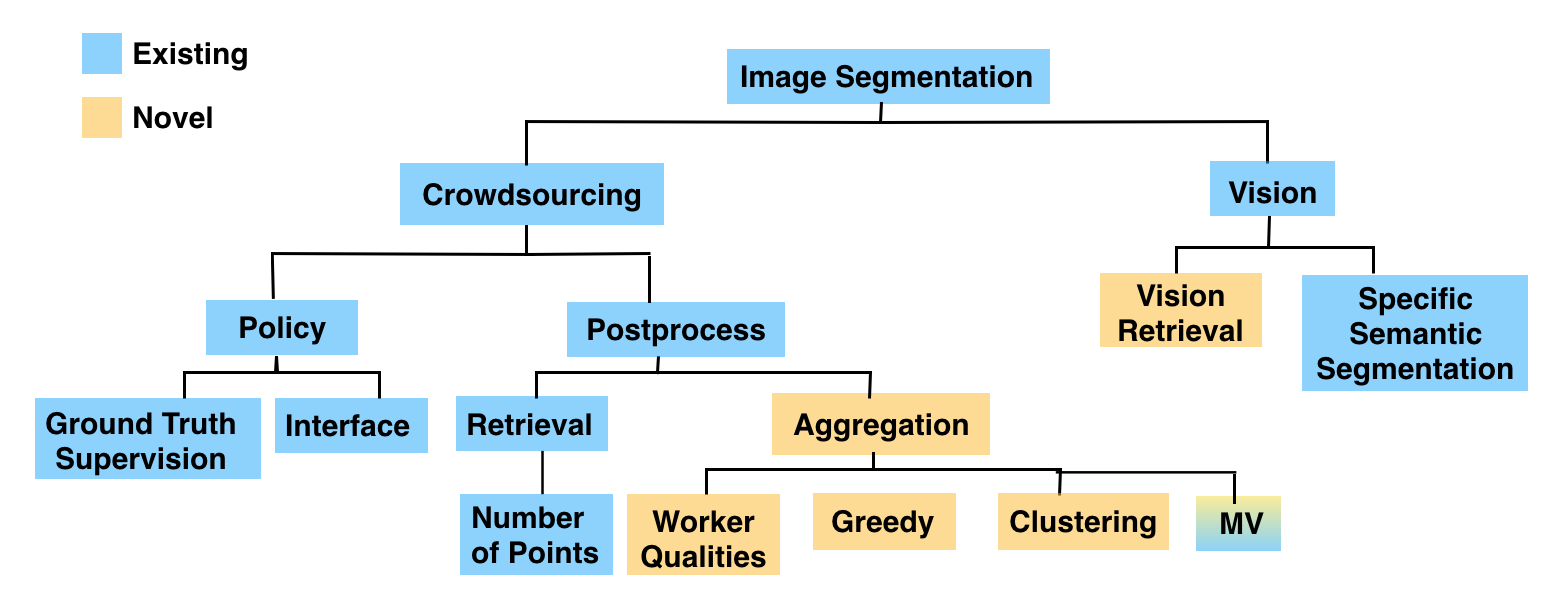
\includegraphics[width=\linewidth]{plots/flowchart.png}
\caption{Flowchart summarizing the classes of existing algorithms for image segmentation (blue) and a novel class of algorithms proposed in this paper (yellow). Majority-vote (MV) is colored both blue and yellow, since a common algorithm in crowdsourcing literature, but have not been extensively applied to crowdsourced image segmentation.}
%The crowdsourced approach can be largely classified as retrieval or aggregation-based methods. We further explore hybrid algorithms that makes use of signals that span over multiple categories, described in our technical report.
\label{flowchart}
\end{figure}
% \agp{I would add textbfs to divide the rest of this up into various clearly defined paragraphs,
% one corresponding to each of your highest levels in the hierarchy
% figure you drew. I would also add one line of introduction at the start.}
Many large-scale efforts in image segmentation contain little to no information on the quality characterization and evaluation of the collected dataset~\cite{Torralba2010,MartinFTM01,Li2009,Gurari2015}, which indicates the lack of standardized approaches for quality evaluation in crowdsourced image segmentation. As shown in Figure \ref{flowchart}, we break down the existing quality evaluation methods into several categories:
\stitle{Policy-based methods}
Policy-based quality evaluation methods are specialized segmentation interfaces or workflows that ensures that the data collected are of good quality. Several large-scale crowdsourced segmentation efforts have employed verification techniques within the data collection workflow, such as supervising workers periodically by evaluating worker responses against known ground-truth segmentation during data collection~\cite{Lin2014,Everingham15}. Common scoring functions for characterize the quality of the worker's segmentation against the ground truth includes segmentation accuracy\cite{Everingham15} or Jaccard index \cite{Sameki2015,Gurari2016}. Specialized interfaces for object segmentation have also been developed to ensure high-quality data collection. For example, Song et al. (\citeyear{Song2018}) makes use of worker's responses from four different image segmentation interfaces to derive an aggregated bounding box. Other segmentation workflows also employ vision information to supervise the crowdsourced response\cite{Russakovsky2015,Gurari2016}. 
%Likewise, Gurari et al. (\citeyear{Gurari2016}) employs a voting-based, hybrid approach making use of expert, crowdsourced and biomedical image segmentation algorithms. 
\par Since these policy-based methods are interface-dependent, require expensive expert-drawn ground-truth annotations or vision information, the results are not easily reproducible. In addition, the segmentations collected by the simple click-and-draw interface in many of the large scale segmentation efforts can not be improved with this technique as a post-processing method. Due to the lack of reproducibility, our paper do not compare against these policy-based methods in extensive details.

\stitle{Retreival-based methods}
Retreival-based methods seeks to pick the ``best'' worker segmentation based on some scoring criteria. \cite{Vittayakorn2011} proposed several heuristic scoring functions that included vision information such as edge detection or color mixture to assess the quality of crowdsourced segmentations.
%Other work~\cite{Sameki2015,Sorokin2008} study the problem of image segmentation for biomedical and natural images. 
\cite{Vittayakorn2011} provides a comparison of retrieval-based algorithms for image segmentation. 
\dor{Need to describe Vittyakorn et al in more detail}
Other heuristic approaches that don't require ground truth segmentations include characterizing the user types and studying their click-stream behavior to determine work quality\cite{Cabezas2015,Sameki2015,Sorokin2008}, and comparing the worker responses to features extracted from computer vision algorithms\cite{Vittayakorn2011,Russakovsky2015}. As we demonstrate in this paper, aggregating worker responses not only eliminates the need for costly expert segmentations, but also leads to better results than individual workers alone.

% \par Despite several large-scale efforts to collect crowdsourced image segmentation~\cite{Lin2014,MartinFTM01,Torralba2010,pascal-voc-2012}, most have relied on summarization-based metrics to quantify their segmentation data quality. 
\par \dor{this paragraph is probably not necessary, if so merge a couple sentence into retreival section}The other methods we evaluated draw on prior work in worker quality evaluation adapted to the segmentation context. Starting from the seminal work of Dawid and Skene~\cite{Dawid1979}, applying Expectation-Maximization (EM) to derive both worker accuracies and true answers\agp{not a complete sentence.}. Welinder and Perona~\cite{OCWelinder2010} extend this \agp{what?} to separately model worker quality and the biases applied to binary, multivalued and continuous annotations. Welinder and Perona~\cite{MDWWelinder2010} develop a multidimensional array of worker accuracies and task difficulties by considering object-presence labeling as a noise generation process\agp{do you mean a noisy generative process?}. The objective truth label is captured by a multidimensional quantity of task-specific measurements and  deformed by worker and image related noise, the noisy vector obtained after this process is projected onto the vector of user expertise (which summarizes how well the user perceives each of these measurements), and finally the score is binarized into an inferred label \agp{fairly confusing and really long sentence}.

\stitle{Aggregation-based methods}
Pixel-based majority vote \agp{since you may not have defined what pixel based majority vote is until this point, i would explicitly describe it} was introduced in \cite{Sameki2015} as a way for aggregating expert-bounding boxes to obtain the ground truth, rather than for aggregating worker segmentations. Many have extended this line of work beyond binary classifications by developing EM-like approaches that works on multiple-choice \cite{Karger2013} as well as free-form responses \cite{Lin2012}, but these have not been directly applied to the task of object segmentation.
\par However, while EM algorithms assign probabilities regarding  \textit{how good a worker's segmentation is}, for the task of object segmentation, we are ultimately more interested the end goal of \textit{what is the best segmentation that we can get from these data}. 
To our knowledge, our work is the first to compare various aggregation-based approaches for segmentation quality evaluation extensively against existing approaches, and study how clustering could be used for the issues of multiple perspectives described in \cite{Sorokin2008,Lin2014,Gurari2018}, for crowdsourced image segmentation\agp{what is described? the issue of perspectives? or clustering?}.

\stitle{Vision-based approaches}
\dor{Describe state-of-the-art precise instance-level segmentation (Facebook Detectron, CRFs). Argue that crowd response is still important}

% Since these formal probabilistic models treats worker bounding box as the base quantity for modeling worker quality, the best bounding box that one could derive from such algorithm can only be as good as the best worker bounding box in the dataset.  Even though the annotation probabilities are sufficient for determining the best binary-labels, image information such as overlapping areas would be useful and not account for in these algorithms. We suspect that this is why many area-based metrics are still more commonly used in practice than EM approaches. \dor{we might not need this paragraph}\agp{not sure of the goal of this para either}